\documentclass[12pt, letterpaper]{article}
\usepackage[utf8]{inputenc}
\usepackage{amsthm}
\usepackage{amsmath}
\usepackage{amsfonts}
\usepackage{amssymb}
\usepackage{mathtools}
\usepackage{tikz}

\title{STA 2503/MMF 1928 Project 1 - American Options}
\author{Siyu Jia, Dixin Mou, Zixun Zhai}
\date{2022/10/01}

\begin{document}
\begin{titlepage}
  \begin{center}
      \vspace*{7cm}

      \textbf{STA 2503/MMF 1928 Project 1 - American Options}

      % \vspace{0.5cm}
      %  Thesis Subtitle
           
      \vspace{1.5cm}

      \textbf{Siyu Jia, Dixin Mou, Zixun Zhai}

      \vfill
           
      % A thesis presented for the degree of\\
      % Doctor of Philosophy
           
      \vspace{0.8cm}
           
      % Department Name\\
      University of Toronto\\
      Toronto, Ontario, Canada\\
      October $1^{st}$, 2022 
           
  \end{center}
\end{titlepage}


\part*{Question 1}
\begin{proof}
We start the proof by considering \[X^{(N)} = \log(\frac{S_T}{S_0}) = \sum_{n=1}^N (r\Delta t+\sigma \sqrt[]{\Delta t} \epsilon_n)\]
The m.g.f of $X^{(N)}$ is: \\
\begin{align*}
  \mathbb{E}^\mathbb{P}[e^{u X^{(N)}}] & =  \mathbb{E}^\mathbb{P}[e^{\sum_{n=1}^N (u r\Delta t+u\sigma \sqrt[]{\Delta t} \epsilon_n)}] \\
  & = \mathbb{E}^\mathbb{P} [\prod_{n=1}^N e^{u r\Delta t+u\sigma \sqrt[]{\Delta t} \epsilon_n}] \\
  & = (\mathbb{E}^\mathbb{P} [e^{u r\Delta t+u\sigma \sqrt[]{\Delta t} \epsilon_1}])^N \tag*{as $\epsilon_n$ is i.i.d}
\end{align*}
We then investigate the inner term $\mathbb{E}^\mathbb{P} [e^{u r\Delta t+ u\sigma \sqrt[]{\Delta t} \epsilon_1}]$:
\begin{align*}
  \mathbb{E}^\mathbb{P} [e^{u r\Delta t+u\sigma \sqrt{\Delta t} \epsilon_1}] &= e^{u r\Delta t +u\sigma \sqrt{\Delta t}} \cdot \frac{1}{2} (1 + \frac{(\mu -r) - \frac{1}{2}\sigma^2}{\sigma} \sqrt{\Delta t}) \\ 
    & \quad + e^{u r\Delta t-u\sigma \sqrt[]{\Delta t}} \cdot \frac{1}{2} (1 - \frac{(\mu -r) - \frac{1}{2}\sigma^2}{\sigma} \sqrt{\Delta t}) \\
    &= [1+u r\Delta t+u \sigma \sqrt{\Delta t} +\frac{1}{2}u^2\sigma^2\Delta t + o(\Delta t)] \cdot \frac{1}{2} (1 + \frac{(\mu -r) - \frac{1}{2}\sigma^2}{\sigma} \sqrt{\Delta t}) \\ 
    & \quad + [1+u r\Delta t-u \sigma \sqrt{\Delta t} +\frac{1}{2}u^2\sigma^2\Delta t + o(\Delta t)] \cdot \frac{1}{2} (1 - \frac{(\mu -r) - \frac{1}{2}\sigma^2}{\sigma} \sqrt{\Delta t}) 
\end{align*}
Note that we collect all the terms containing $\Delta t$ with order 2 or higher to be $o(\Delta t)$ because as $N\rightarrow \infty$ 
and $\Delta t \rightarrow 0$, $o(\Delta t)$ will converge to 0 faster than $\Delta t$ or $\Delta t$ with lower orders.
\\ \\ 
We then continue the algebra manipulation:
\begin{align*}
  \mathbb{E}^\mathbb{P} [e^{u r\Delta t+u\sigma \sqrt{\Delta t} \epsilon_n}] &= [1+u r\Delta t+u \sigma \sqrt{\Delta t} +\frac{1}{2}u^2\sigma^2\Delta t + o(\Delta t)] \cdot \frac{1}{2} (1 + \frac{(\mu -r) - \frac{1}{2}\sigma^2}{\sigma} \sqrt{\Delta t}) \\ 
    & \quad + [1+u r\Delta t-u \sigma \sqrt{\Delta t} +\frac{1}{2}u^2\sigma^2\Delta t + o(\Delta t)] \cdot \frac{1}{2} (1 - \frac{(\mu -r) - \frac{1}{2}\sigma^2}{\sigma} \sqrt{\Delta t}) \\
    &= \frac{1}{2}[ 1 + \frac{(\mu - r) - \frac{1}{2}\sigma^2}{\sigma}\sqrt{\Delta t} + u r \Delta t + u \sigma \sqrt{\Delta t} \\
    & \quad + u((\mu -r) - \frac{1}{2}\sigma^2)\Delta t + \frac{1}{2}u^2 \sigma^2 \Delta t \\
    & \quad + 1 - \frac{(\mu - r) - \frac{1}{2}\sigma^2}{\sigma}\sqrt{\Delta t} + ur \Delta t - u\sigma \sqrt{\Delta t} \\
    & \quad + u((\mu -r) - \frac{1}{2}\sigma^2)\Delta t + \frac{1}{2}u^2 \sigma^2 \Delta t + o(\Delta t)] \\
    &= 1 + ur \Delta t + u((\mu - r) - \frac{1}{2}\sigma^2)\Delta t + \frac{1}{2}u^2 \sigma^2 \Delta t + o(\Delta t) \\
    &= 1 + (ur + u\mu - ur -\frac{1}{2}u \sigma^2 + \frac{1}{2}u^2 \sigma^2)\Delta t + o(\Delta t) \\
    &= 1 + (u (\mu - \frac{1}{2}\sigma^2) + \frac{1}{2}u^2 \sigma^2)\Delta t + o(\Delta t)\\
    &= e^{(u (\mu - \frac{1}{2}\sigma^2) + \frac{1}{2}u^2 \sigma^2)\Delta t} + o(\Delta t)
\end{align*} 
As a result:
\begin{align*}
  \mathbb{E}^\mathbb{P}[e^{u X^{(N)}}] & = (e^{(u (\mu - \frac{1}{2}\sigma^2) + \frac{1}{2}u^2 \sigma^2)\Delta t} + o(\Delta t))^N\\
    &=  e^{(u(\mu - \frac{1}{2}\sigma^2)T + \frac{1}{2}u^2 \sigma^2T)} \tag*{as $N \rightarrow \infty$ and $\Delta t = \frac{T}{N}$}
\end{align*}
We notice that the m.g.f of the $X^{(N)}$ is equal to the m.g.f of a random variable $Y$ whcih follows the normal distribution with mean to be $(\mu - \frac{1}{2}\sigma^2)T$ and
variance to be $\sigma^2 T$.
\\ \\
Thus, we prove that:
\[X^{(N)} \xrightarrow[N \rightarrow \infty]{d} (\mu - \frac{1}{2}\sigma^2)T + \sigma^2 TZ\]
where 
\[Z \stackrel{\mathbb{P}}{\sim} \mathcal{N}(0, 1)\] 
\end{proof}

\part*{Question 2}
\section*{Part 1}
We firstly find the martingale measure $\mathbb{Q}(\epsilon_k = \pm 1)$ where $\mathbb{Q}(\epsilon_k =1) = q_k$ and $\mathbb{Q}(\epsilon_k =-1) = 1-q_k$. Consider 
time $t_k$ and $t_{k+1}$, we have the following for $B$ and $S$. \\ \\ 
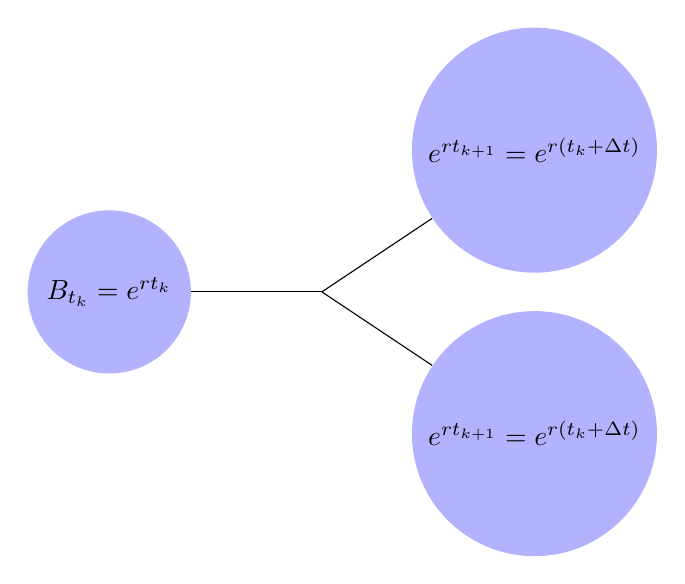
\begin{tikzpicture}[level distance=30mm,sibling distance=40mm,every node/.style={fill=blue!30,circle,inner sep=5pt}, scale = 0.9]
  \node {$B_{t_k} = e^{rt_k}$}
  child[grow=right] {
  child {node{$e^{rt_{k+1}} = e^{r(t_k + \Delta t)}$}} child {node{$e^{rt_{k+1}} = e^{r(t_k + \Delta t)}$}}
  };
\end{tikzpicture}
\\
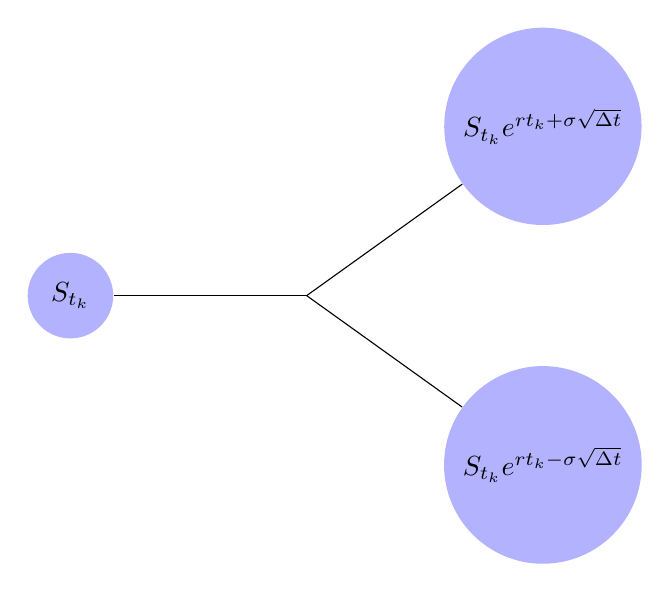
\begin{tikzpicture}[level distance=30mm,sibling distance=43mm,every node/.style={fill=blue!30,circle,inner sep=5pt}]
  \node {$S_{t_k}$}
  child[grow=right] {
  child {node{$S_{t_k}e^{rt_k-\sigma \sqrt{\Delta t}}$}} child {node{$S_{t_k}e^{rt_k+\sigma \sqrt{\Delta t}}$}}
  };
\end{tikzpicture}\\
We construct the following $\mathbb{Q}$-martingale:
\begin{align*}
&\qquad \frac{S_{t_k}}{e^{rt_k}} = q_k\frac{S_{t_k}e^{r\Delta t + \sigma \sqrt{\Delta t}}}{e^{r(t_k+\Delta t)}} + (1-q_k)\frac{S_{t_k}e^{r\Delta t - \sigma \sqrt{\Delta t}}}{e^{r(t_k+\Delta t)}}\\
&\Rightarrow 1 = q_k\frac{e^{r\Delta t + \sigma \sqrt{\Delta t}}}{e^{r\Delta t}} + (1-q_k) \frac{e^{r\Delta t - \sigma \sqrt{\Delta t}}}{e^{r\Delta t}} \\
&\Rightarrow q_k(e^{r\Delta t + \sigma \sqrt{\Delta t}} - e^{r\Delta t - \sigma \sqrt{\Delta t}}) = e^{r\Delta t} - e^{r\Delta t - \sigma \sqrt{\Delta t}} \\
&\Rightarrow q_k = q = \frac{e^{r\Delta t} - e^{r\Delta t - \sigma \sqrt{\Delta t}}}{e^{r\Delta t + \sigma \sqrt{\Delta t}} - e^{r\Delta t - \sigma \sqrt{\Delta t}}} \tag*{As $q_k$ does not depend on $k$}
\end{align*} 
\\
We then Taylor-expand the exponential terms and collect all all the terms containing $\Delta t$ with order 2 or higher to be $o(\Delta t)$:
\begin{align*}
  q &= \frac{e^{r\Delta t} - e^{r\Delta t - \sigma \sqrt{\Delta t}}}{e^{r\Delta t + \sigma \sqrt{\Delta t}} - e^{r\Delta t - \sigma \sqrt{\Delta t}}}\\
  &= \frac{1+r\Delta t - (1 + r \Delta t - \sigma \sqrt{\Delta t} + \frac{1}{2} \sigma^2\Delta t) + o(\Delta t)}
    {1+r\Delta t + \sigma \sqrt{\Delta t} + \frac{1}{2} \sigma^2\Delta t - (1 + r \Delta t - \sigma \sqrt{\Delta t} + \frac{1}{2} \sigma^2\Delta t) + o(\Delta t)} \\
  &= \frac{\sigma \sqrt{\Delta t} - \frac{1}{2} \sigma^2\Delta t + o(\Delta t)}{2\sigma\sqrt{\Delta t} + o(\Delta t)}\\
  &= \frac{1}{2} - \frac{1}{4}\sigma\sqrt{\Delta t} + o(\sqrt{\Delta t}) \\
  &= \frac{1}{2}(1 - \frac{1}{2}\sigma\sqrt{\Delta t}) + o(\sqrt{\Delta t})
\end{align*}

\newpage
\section*{Part 2}
Similarly, we want to find the martingale measure $\mathbb{Q}^S(\epsilon_k = \pm 1)$ where $\mathbb{Q}^S(\epsilon_k =1) = h_k$ and $\mathbb{Q}^S(\epsilon_k =-1) = 1-h_k$. Consider 
time $t_k$ and $t_{k+1}$, this time we use $S$ as the numeraire. \\ \\
We construct the following $\mathbb{Q}^S$-martingale:
\begin{align*}
  &\qquad \frac{e^{rt_k}}{S_{t_k}} = h_k\frac{e^{r(t_k+\Delta t)}}{S_{t_k}e^{r\Delta t + \sigma \sqrt{\Delta t}}} + (1-h_k)\frac{e^{r(t_k+\Delta t)}}{S_{t_k}e^{r\Delta t - \sigma \sqrt{\Delta t}}}\\
  &\Rightarrow  1 = h_k\frac{e^{r\Delta t}}{e^{r\Delta t + \sigma \sqrt{\Delta t}}} + (1-h_k) \frac{e^{r\Delta t}}{e^{r\Delta t - \sigma \sqrt{\Delta t}}} \\
  &\Rightarrow e^{2r\Delta t} = h_ke^{2r\Delta t - \sigma \sqrt{\Delta t}} + (1-h_k)e^{2r\Delta t + \sigma \sqrt{\Delta t}}\\
  &\Rightarrow e^{2r\Delta t} - e^{2r\Delta t + \sigma \sqrt{\Delta t}} = h_k(e^{2r\Delta t - \sigma \sqrt{\Delta t}} - e^{2r\Delta t + \sigma \sqrt{\Delta t}}) \\
  &\Rightarrow h_k = h = \frac{e^{2r\Delta t} - e^{2r\Delta t + \sigma \sqrt{\Delta t}}}{e^{2r\Delta t - \sigma \sqrt{\Delta t}} - e^{2r\Delta t + \sigma \sqrt{\Delta t}}} \tag*{As $h_k$ does not depend on $k$}
\end{align*}
We then Taylor-expand the exponential terms and collect all all the terms containing $\Delta t$ with order 2 or higher to be $o(\Delta t)$:
\begin{align*}
  h &= \frac{e^{2r\Delta t} - e^{2r\Delta t + \sigma \sqrt{\Delta t}}}{e^{2r\Delta t - \sigma \sqrt{\Delta t}} - e^{2r\Delta t + \sigma \sqrt{\Delta t}}} \\
    &= \frac{1+2r\Delta t - (1+2r\Delta t+\sigma \sqrt{\Delta t} + \frac{1}{2} \sigma^2\Delta t) + o(\Delta t)}
        {1+2r\Delta t - \sigma \sqrt{\Delta t} + \frac{1}{2} \sigma^2\Delta t - (1+2r\Delta t+\sigma \sqrt{\Delta t} + \frac{1}{2} \sigma^2\Delta t) + o(\Delta t)}\\
    &= \frac{-\sigma \sqrt{\Delta t} - \frac{1}{2} \sigma^2\Delta t+ o(\Delta t)}{-2\sigma \sqrt{\Delta t} +o(\Delta t)}\\
    &= \frac{\sigma \sqrt{\Delta t} + \frac{1}{2} \sigma^2\Delta t+ o(\Delta t)}{2\sigma \sqrt{\Delta t} +o(\Delta t)}\\
    &= \frac{1}{2}(1+\frac{1}{2}\sigma \sqrt{\Delta t}) + o(\sqrt{\Delta t})
\end{align*}


\end{document}